\documentclass[main.tex]{subfiles}

\begin{document}

\subsection{Primo esercizio}

\begin{figure}[H]
\centering
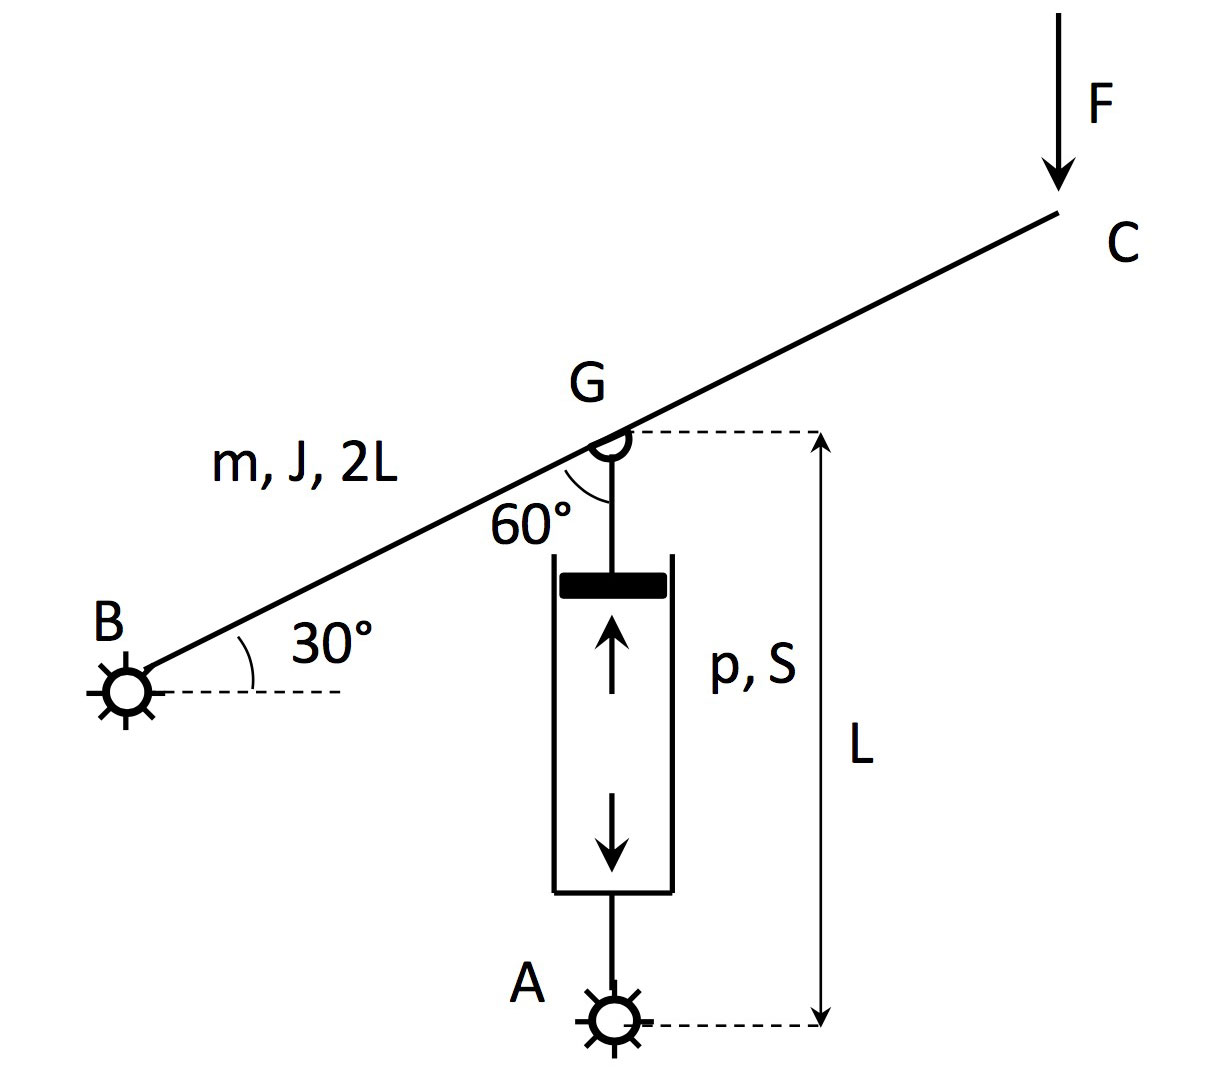
\includegraphics[width=0.75\textwidth]{2014-0407-1.jpg}
\end{figure}

\[
	L = 2\,m \quad
	S = 0.02\,m^2 \quad
	m = 200\,kg \quad
	J = 50\,kg m^2 \quad
	v = 0.2\,m/s \quad
	F = 5000\,N \quad
\]

Il sistema rappresentato in figura è posto nel piano verticale. L'asta BC è vincolata a terra con una cerniera in B e ha massa $m$, momento d'inerzia baricentrico $J$ e lunghezza $2L$. A tale asta, nel baricentro G (posto a metà dell'asta), è collegato un attuatore idraulico (di massa trascurabile), il cui estremo inferiore è incernierato a terra in A. Si consideri pari a S l'area del pistone e pari a p la pressione dell’olio nell'attuatore (si ricorda che le due forze uguali ed opposte esercitate dall’olio sul cilindro e sul pistone hanno modulo pari a $p*S$).
Nella posizione considerata, la lunghezza complessiva dell'attuatore è pari ad $L$. Sull'asta BC, nel punto C, agisce una forza $F$, diretta come in figura.

Nota la geometria del sistema e assegnate la forza F e la velocità $v$ di sfilo dell'attuatore (costante), si chiede di calcolare:
\begin{enumerate}
\item La velocità e l’accelerazione del punto C.
\item La pressione dell’olio all'interno dell'attuatore, necessaria per garantire la condizione di moto assegnata.
\end{enumerate}

\clearpage

\subsection{Soluzione primo esercizio}

\subsubsection{Primo punto}
la velocità e l'accelerazione del punto C possono essere definite tramite i legami cinematici con l'accelerazione e velocità angolare di B.
\\
\paragraph{Equazione di chiusura} Utilizzo come equazione di chiusura (B-G) + (G-A) = (B-A)

Definisco $b = BG$, $a = GA$ e $c = BA$, mentre $\beta = \dfrac{\pi}{6}$ come l'angolo che descrive l'orientamente del segmento BG, $\alpha = \dfrac{3\pi}{2}$ quello del segmento GA e $\gamma$ quello del segmento BA.

\paragraph{Spostamento}

\[
	be^{i\beta} + ae^{i\alpha} = ce^{i\gamma}
\]

Scompongo in componenti cartesiane:

\[
	\begin{cases}
		b\sin\beta + a\sin\alpha = c\sin\gamma\\
		b\cos\beta + a\cos\alpha = c\cos\gamma\\
	\end{cases}
	\Longrightarrow
	\begin{cases}
		\gamma = \arctan\left (\dfrac{b\sin\beta + a\sin\alpha}{b\cos\beta + a\cos\alpha}\right ) = -\dfrac{\pi}{3}rad\\
		c = \dfrac{b\cos\beta + a\cos\alpha}{\cos\gamma}=3.46\,m\\
	\end{cases}
\]

\paragraph{Velocità} Derivo ed ottengo le velocità, tenendo a mente che $\beta$, $\alpha$ e $a$ sono variabili nel tempo.

\[
	b\dot{\beta}e^{i\left ( \dfrac{\pi}{2} + \beta \right )} + \dot{a}e^{i\alpha} + a\dot{\alpha}e^{i\left ( \dfrac{\pi}{2} + \alpha \right )} = 0
\]

Scompongo in componenti cartesiane:

\[
\begin{cases}
	b\dot{\beta}\cos\beta + \dot{a}\sin\alpha + a\dot{\alpha}\cos\alpha = 0 \\
	- b\dot{\beta}\sin\beta + \dot{a}\cos\alpha - a\dot{\alpha}\sin\alpha = 0 \\
\end{cases}
\]

Siccome $\cos\alpha = 0$ in questo caso, e $v = -\dot{a} = 0.2\,m/s$  posso semplificare il sistema:

\[
\begin{cases}
	b\dot{\beta}\cos\beta + \dot{a}\sin\alpha = 0 \\
	- b\dot{\beta}\sin\beta - a\dot{\alpha}\sin\alpha = 0 \\
\end{cases}
\Longrightarrow
\begin{cases}
	\dot{\beta} = \dfrac{\dot{a}\sin\alpha}{b\cos\beta} = 0.11\,rad/s \\
	 \dot{\alpha}= -\dfrac{b\dot{\beta}\sin\beta}{a\sin\alpha} = 0.06\,rad/s \\
\end{cases}
\]

\paragraph{Accelerazione} Derivo nuovamente ed ottengo l'accelerazione, tenendo presente che $\beta$, $\dot{\beta}$, $\alpha$, $\dot{\alpha}$ e $a$ sono variabili nel tempo.

\[
	b\ddot{\beta}e^{i\left ( \dfrac{\pi}{2} + \beta \right )} - b\dot{\beta}^2e^{i\beta} + a\ddot{\alpha}e^{i\left ( \dfrac{\pi}{2} + \alpha \right )} - a\dot{\alpha}^2e^{i\alpha} = 0
\]

Scompongo in componenti cartesiane:

\[
\begin{cases}
\end{cases}
\]

\end{document}
